\section{Experimento 4} 

En este experimento se utilizará un circuito sencillo para generar una señal de amplitud modulada. El circuito emplea un circuito
sintonizado, cuyos valores se han elegido para que resuene aproximadamente a \(50\,\mathrm{kHz}\).

Para realizar esta experiencia se necesitarán dos generadores de señales. Uno de ellos deberá
entregar una señal senoidal, que funcionará como portadora. El otro se utilizará para generar una señal moduladora.

\begin{figure}[H]
    \centering
    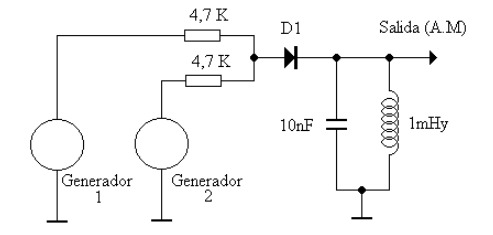
\includegraphics[width=0.4\textwidth]{images/esquemaE4.jpeg}
    \caption{Esquema del circuito del experimento 4}
\end{figure}

Luego de conectar se realiza la configuración de los generadores de señales considerando los siguientes parámetros:

\begin{itemize}
    \item Generador de señal portadora: \(f_c = 50\,\mathrm{kHz}\), media vuelta el control de
nivel de salida.
    \item Generador de señal moduladora: \(f_m = 1\,\mathrm{kHz}\), un cuarto de vuelta el
control de nivel de salida.
\end{itemize}
Con la configuración correcta del osciloscopio se puede ver la señal como una  superposición de trazos de varias amplitudes. 

\begin{figure}[H]
    \centering
    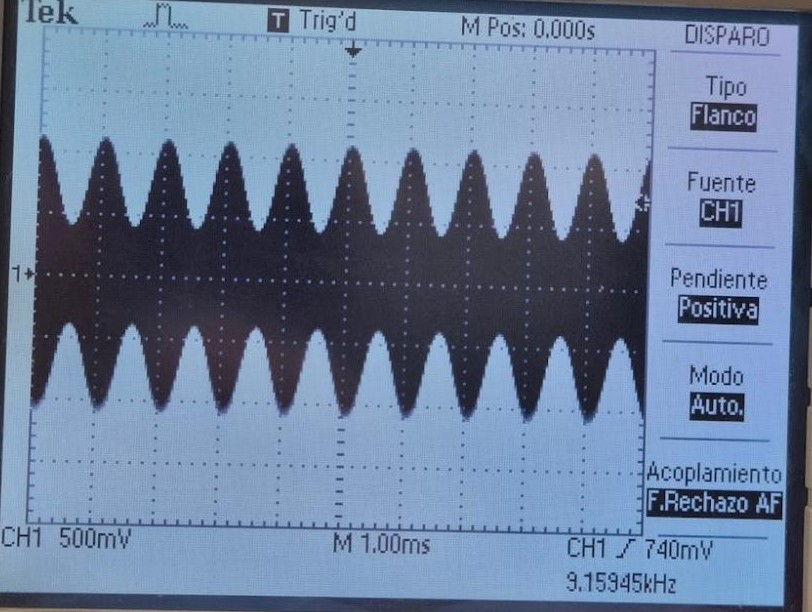
\includegraphics[width=0.4\textwidth]{images/image1.jpg}
    \caption{Señal modulada en el dominio del tiempo}
\end{figure}
 Se ajustará el osciloscopio para visualizarla claramente en la pantalla la señal modulada en el dominio de la frecuencia. 

 Para ello, en el modo ``Math Menu'' se seleccionará la ventana ``Hanning'' y la operación ``FFT'', lo que permitirá observar la señal modulada en el dominio de la frecuencia.Usando los cursores del osciloscopio, se puede determinar la frecuencia de la portadora y la de sus bandas laterales. Se obtienen los siguientes valores:
 \begin{figure}[H]
    \centering
    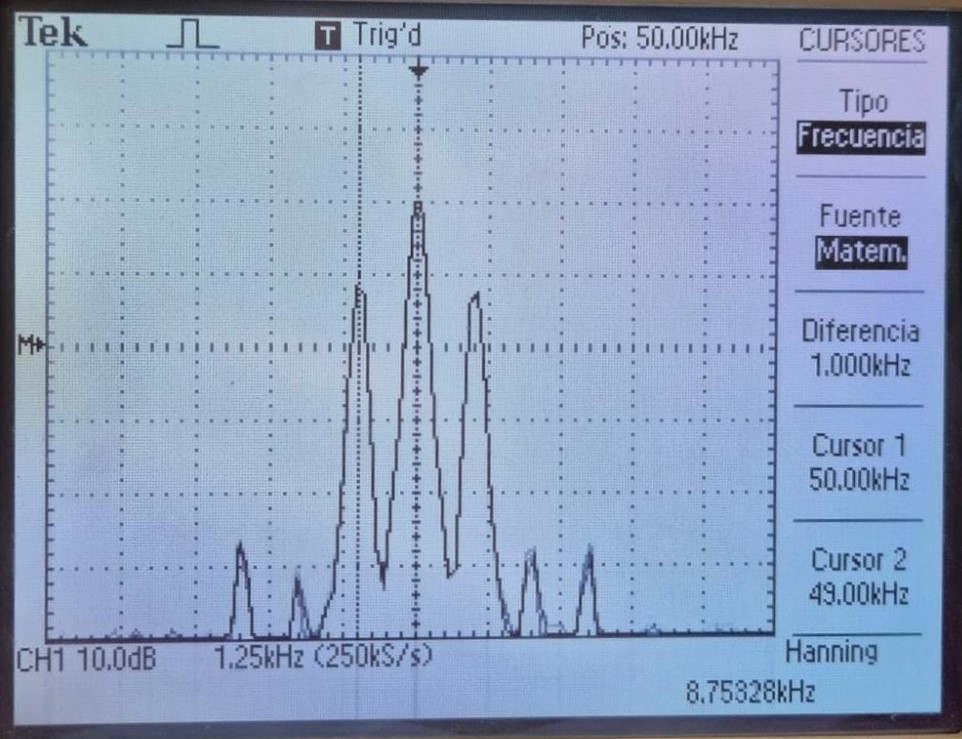
\includegraphics[width=0.4\textwidth]{images/image6.jpg}
    \caption{Señal modulada en el dominio de la frecuencia}
\end{figure}

\begin{center}
\begin{tabular}{@{}c@{}}
Frec. portadora (Port):
\underline{\hspace{0.2cm}$50\,\mathrm{kHz}$\hspace{0.2cm}}
\\[0.25cm]

Frec. lateral sup./inf. (F\textsubscript{L}):
\underline{\hspace{0.2cm}$49\,\mathrm{kHz}$\hspace{0.2cm}}
\\[0.25cm]

Frec. modulante (Dif.):
\underline{\hspace{0.2cm}$1\,\mathrm{kHz}$\hspace{0.2cm}}
\end{tabular}
\end{center}
Se puede realizar el mismo análisis para determinar la amplitud de la portadora y de las bandas laterales con los cursores en ``Amplitud''. Se obtienen los siguientes valores:
 \begin{figure}[H]
    \centering
    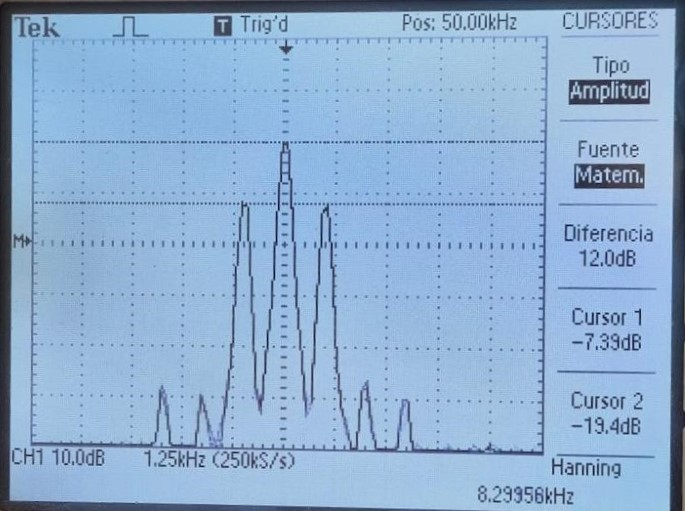
\includegraphics[width=0.4\textwidth]{images/image4.jpg}
    \caption{Señal modulada en el dominio de la frecuencia con su amplitud}
\end{figure}
\begin{center}
\begin{tabular}{@{}c@{}}
Amplitud portadora (Port):
\underline{\hspace{0.2cm}$-7.39\,\mathrm{dB}$\hspace{0.2cm}}
\\[0.25cm]
Amplitud lateral sup./inf. (L):
\underline{\hspace{0.2cm}$-19.4\,\mathrm{dB}$\hspace{0.2cm}}
\\[0.25cm]
Amplitud modulante (Dif.):
\underline{\hspace{0.2cm}$12\,\mathrm{dB}$\hspace{0.2cm}}
\end{tabular}
\end{center}
Conociendo la amplitud de la portadora y de las bandas laterales, se puede calcular el índice de modulación \(m\) mediante la siguiente fórmula:
\begin{gather*}
m_{\mathrm{dB}} = -19{,}4 - (-7{,}39) + 6 = -6{,}01\,\mathrm{dB} \\[1ex]
m = 10^{\frac{-6{,}01}{20}} \approx 0{,}50
\end{gather*}
Se puede observar tambien que la señal modulada varia dependiendo de la forma de onda de la señal modulante. A continuación se muestran las señales moduladas en el dominio del tiempo y de la frecuencia para una señal modulante triangular y una señal modulante cuadrada.
 \begin{figure}[H]
    \centering
    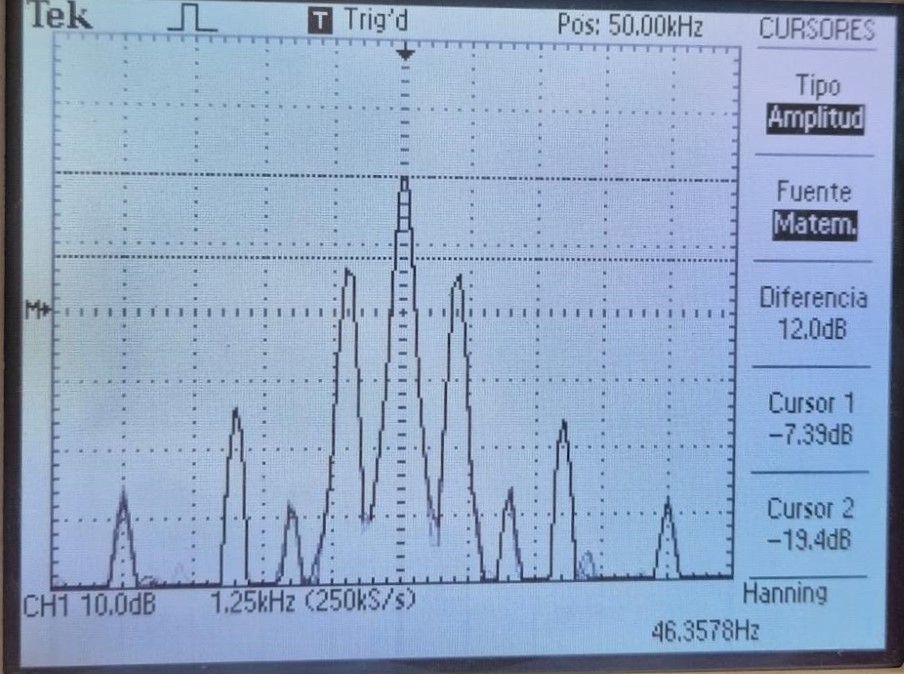
\includegraphics[width=0.4\textwidth]{images/image14.jpg}
    \caption{Señal modulante triangular}
\end{figure}
 \begin{figure}[H]
    \centering
    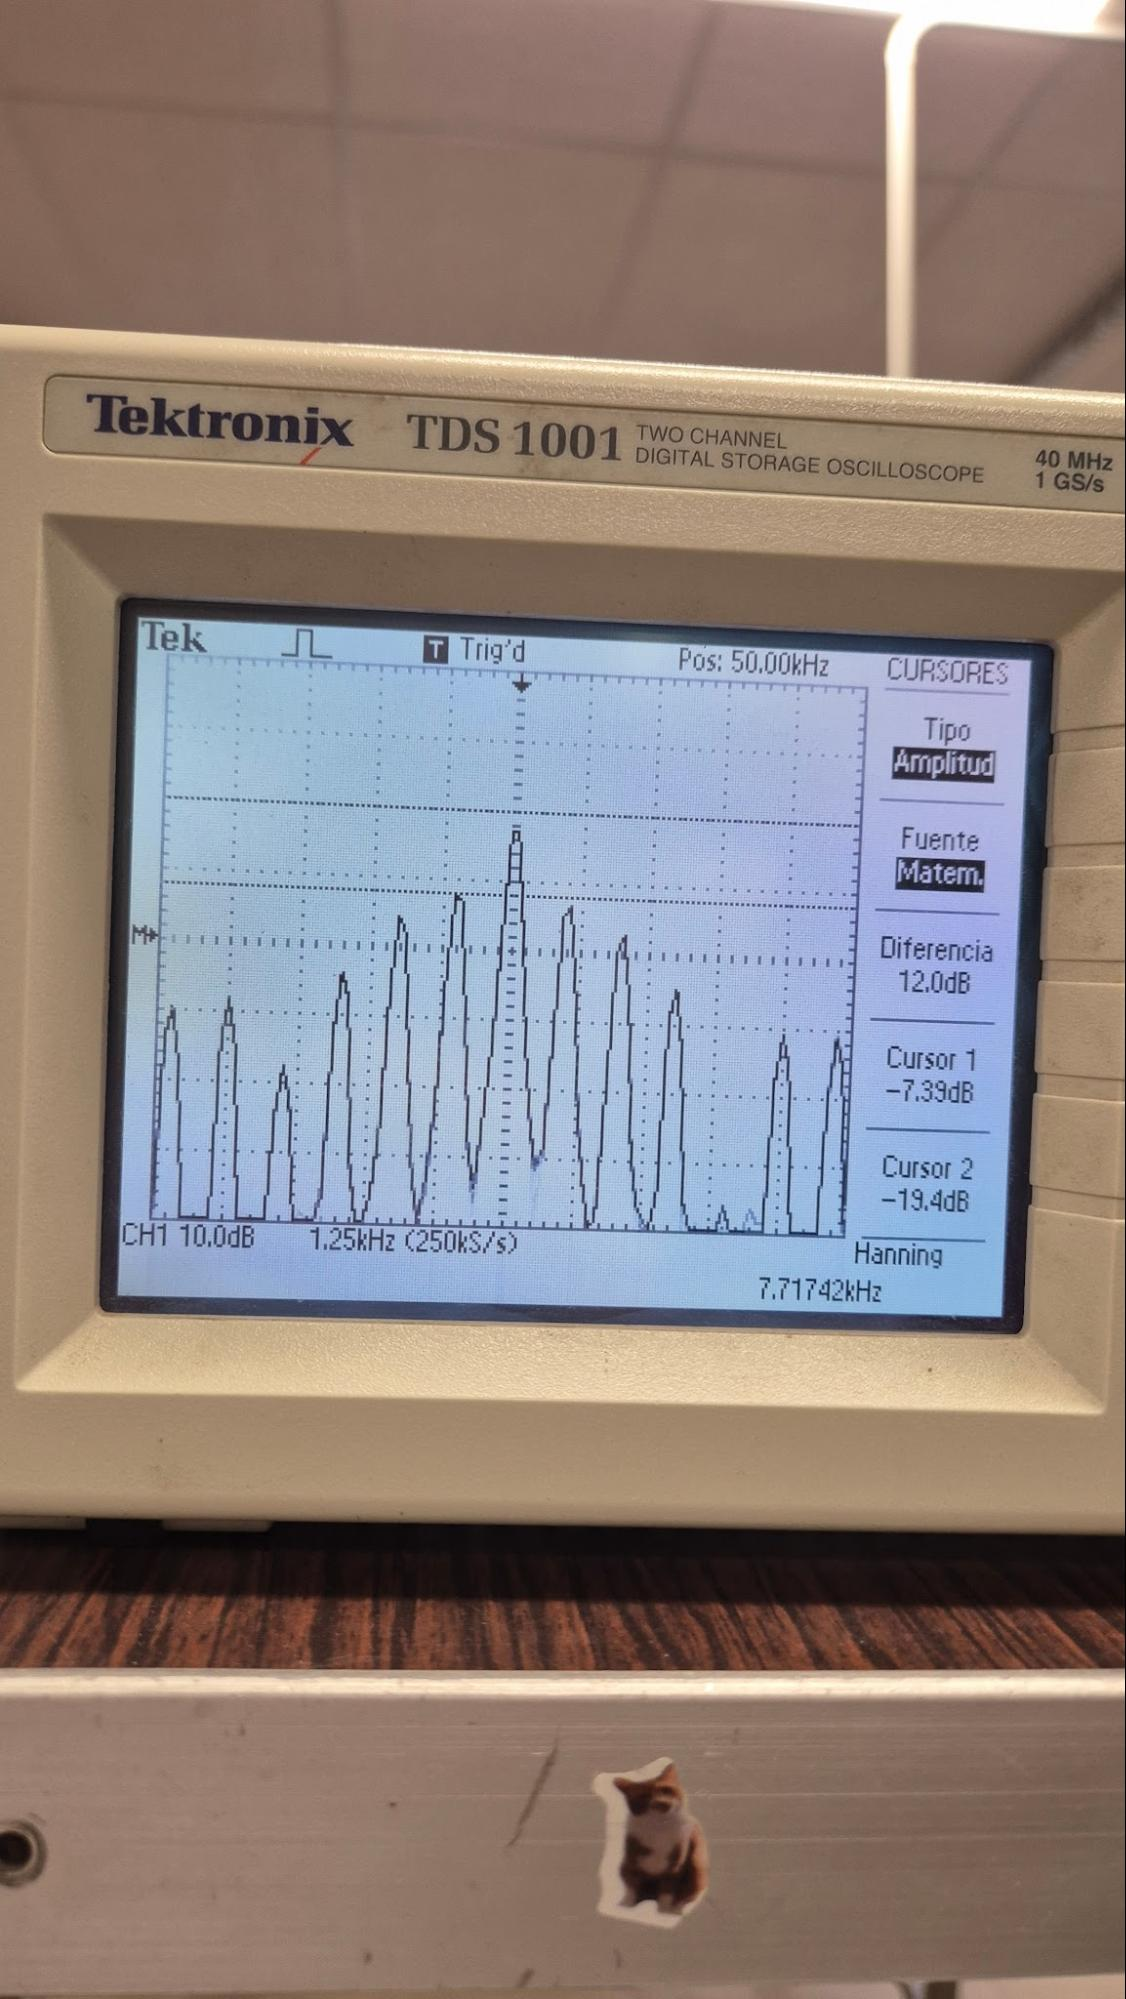
\includegraphics[width=0.4\textwidth]{images/image5.jpg}
    \caption{Señal modulante cuadrada}
\end{figure}
